\chapter{Protocol messages}
In this chapter we describe different protocol messages in detail. For
readability the protocol messages are presented before their presentation is
encoded into BSON.


% Values for type:
% 0: List
% 1: List reply
% 2: Subscribe
% 3: Subscribe ack
% 4: Update
% 5: Update ack
% 6: Unsubscribe
% 7: Keep-alive

\section{Listing available sensors}
With \texttt{list} message type a client can retrieve a list of available
sensors publishing updates into the server. The request has a following
presentation:
\\
\\
\texttt{\{'type': integer\}}
\\
\\
The value of \texttt{type} key for list message must contain an integer value 0.


The \texttt{list response} message contains a list of available sensor IDs and
has a following presentation:
\\
\\
\texttt{\{'type': integer, 'sids': [string, ...]\}}
\\
\\
The value of \texttt{type} key for list response message must contain an integer
value 1. The value of \texttt{sids} key contains a list of strings interpreted
as sensor IDs.


\section{Subscribing}
In order to receive updates from a specific sensor the client must subscribe to
that sensor with a \texttt{subscribe} message. The message takes a list
of elements describing the sensor id and whether or not the updates are 
to be delivered in a reliable manner.

% TODO I think we should put this into a separate 'Operation logic' chapter

\includegraphics[scale=0.75, trim= 100 0 50 0]{subscribe.pdf}

% Shall we prefer readability or minimal overhead 
% BSON is not readable anyway, and I think we are on it because of minimal overhead
% for binary data
% - Yeah, let's think this in future. Currently lots of bits wasted on long
%   keys in BSON objects.

The subscribe message sent by the client has the following format:
\\
\\
\texttt{\{'type': integer, 'sids': [\{'id': string, 'reliable': integer\}, ...]\}}
\\
\\
The value of \texttt{type} key for subscribe message must contain an integer
value 2. The value of \texttt{sids} key contains a list of sensor objects. Each of the sensor
objects have a key \texttt{id} with a string of the sensor id as a value and optional
\texttt{reliable} key with a boolean value.

The subscribe acknowledgement from the server has the following format:
\\
\\
\texttt{\{'type': integer, 'sids': [\{'id': string, 'status': integer\}, ...]\}}
\\
\\
The value of \texttt{type} key for subscribe acknowledgement must contain an
integer value 3. The value of \texttt{sids} key contains a list of sensor objects. Each of the sensor
objects have a key \texttt{id} with a string of the sensor id as a value and
\texttt{status} key with an integer value as a return value. If the subscription
was successful the return value must be 0. Other values indicate different error
reasons. When the sensor does not exist the return value is 1. If the client is
already subscribed, the return value is 2.
% XXX: Other reasons
% Do you think it's good to adopt HTTP return values?
% - It sounds a little funny and we have no reason to use this except the one
%   that HTTP uses the same coding. However we can still 

\section{Receiving updates}
The updates from sensors are delivered to clients with \texttt{update} messages. Depending on
the subscribe parameters the update delivery can be either reliable or
unreliable.

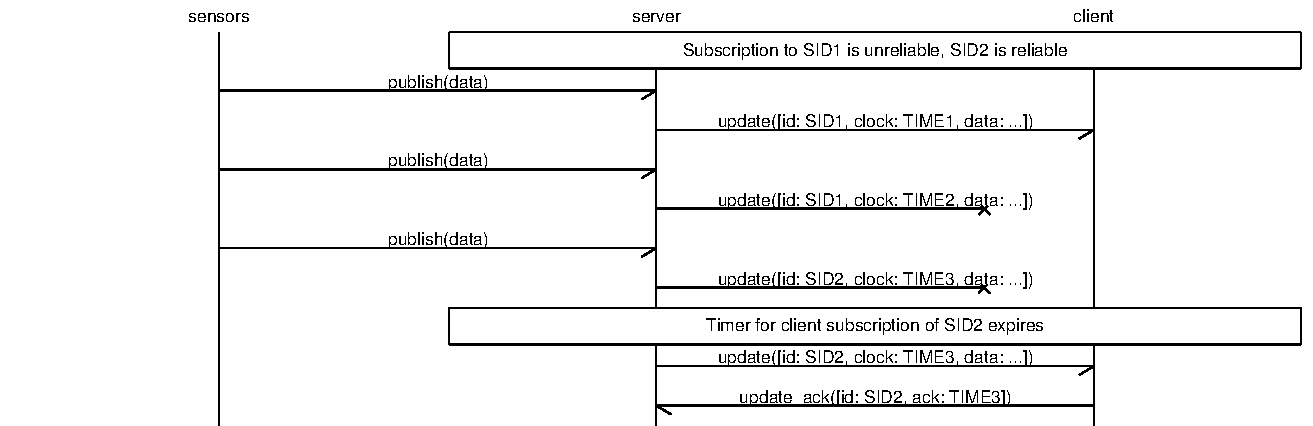
\includegraphics[scale=0.7, trim=125 0 50 0]{update.pdf}

The message has the following format before it is encoded into a binary form:
\\
\\
\texttt{\{'type': integer, 'sid': string, 'sensor\_type': integer, 'time':
integer, 'reliable': boolean, 'data': sensor\_data\}}
\\
\\
The value of \texttt{type} key for update message must contain an integer value
4. The value of \texttt{sid} key is a string presentation of the sensor id. the
\texttt{sensor\_type} key is used to hold the information about the type of the
sensor. Possible values are 0 for status sensors, 1 for temperature sensors, 2
for GPS sensors, and 3 for camera sensors. The value of \texttt{time} key holds
an integer value (protocol clock) used with reliable transport. The value of
\texttt{reliable} key indicates whether or not the client must acknowledge this
update. The value of \texttt{data} contains the actual data from sensor. This
can be boolean (status sensors), float (temperature sensors), string (GPS), or
binary (camera) data depending on the sersor type of the message.
% sensor_type:
% 0: Status
% 1: Temperature
% 2: GPS
% 3: Camera
% sensor_data can be interpreted based on the sensor_type
% For type 0: boolean
%          1: float
%          2: string
%          3: binary

If the transmission is reliable and it is stated in the update message then the
client must send the update acknowledgment.

The update acknowledgment message has the following format:
\\
\\
\texttt{\{'type': integer, 'sid': string, 'sensor\_type': integer, 'time': integer\}}
\\
\\

The value of \texttt{type} key for the update acknowledgment message must contain an integer value
5. The value of keys \texttt{sid}, \texttt{sensor\_type} and \texttt{time} must
be the same as in the update message.

The client may also support negative acknowledgements which are sent when the
client detects a packet loss from cap in the message sequence numbers. This
message is sent to server to inform it that a loss has occured.

The negative updata acknowledgement message has the following format:
\\
\\
\texttt{\{'type': integer, 'sid': string, 'seq\_no': integer\}}
\\
\\


\section{Unsubscribing}
When a client wants to end the receiving of updates from a specific sensor it
sends a \texttt{unsubscribe} message to the server. Upon receiving the
\texttt{unsubscribe} message from a client the server removes the client from
the recipient list of the specific sensor IDs given in the unsubscribe message.

The unsubscribe message sent by the client has the following format:
\\
\\
\texttt{\{'type': integer, 'sids': [\{'id': string\}, ...]\}}
\\
\\
The value of \texttt{type} key for the unsubscribe message must contain an integer value
6. The value of \texttt{sids} key contains a list of sensor objects. Each of the sensor
objects have a key \texttt{id} with a string of the sensor id as a value.

\section{Keep-alive messaging}
The clients must send \texttt{keep-alive} messages with constant pace to server. From the
absence of these keep-alive messages the server can infer the dead clients and
can safely remove these from its receiver lists.

The keep-alive message sent by the client has the following format:
\\
\\
\texttt{\{'type': integer\}}
\\
\\
The value of \texttt{type} key for the keep-alive message must contain an
integer value 7.


%Arseny: lets not introduce this ACK. Rather we can have small keep-alive at client like 1 second
%And quite big constant at the server, like 10. Well I put 5s and 5. Rather randomly.
%The server must acknowledge to client when a keep-alive message is received and client should
%retransmit the keep-alive message to server if it does not receive the acknowledgement from server. 

%Error codes for acknowledments
%\begin{table}[htb]
%\begin{tabular}{|c|l|}
%\hline
%E\_NOT\_SUBSCRIBED & the client has no active subscriptions in the server \\
%\hline
%\end{tabular}
%\end{table}

